\documentclass[a4paper,12pt]{report}

\usepackage{alltt, fancyvrb, url}
\usepackage{graphicx}
\usepackage[utf8]{inputenc}
\usepackage{float}
\usepackage{hyperref}

% Questo commentalo se vuoi scrivere in inglese.
\usepackage[italian]{babel}

\usepackage[italian]{cleveref}

\title{Relario: Tales of Relano\\Progetto per il corso di\\``Programmazione ad Oggetti''}

\author{Lorenzo Cinelli, Mihai Mazuru, Kimi Osti, Sara Panfini}
\date{\today}


\begin{document}

\maketitle

\tableofcontents

\chapter{Analisi}


\section{Descrizione e requisiti}

Il software realizzato è un videogioco 2D con vista dall’alto. Il suo svolgimento gira attorno a un personaggio principale, controllato dall’utente, che deve attraversare le stanze di un castello per raggiungere lo scontro finale con il Re, di cui deve conquistare il trono.
%
\newline Durante l’esplorazione delle stanze all’utente potranno essere affidate delle quest da completare per poter procedere correttamente.
%
\newline Inoltre, gli verranno presentato delle stanze quasi completamente interattive. In particolare, ci saranno dei personaggi non giocanti (neutri, alleati o nemici) che potranno, al momento dell’interazione, mostrare un messaggio, donare degli oggetti oppure ingaggiare un combattimento. Inoltre, sarà possibile interagire con gran parte degli elementi di arredo presenti in stanza, tra cui elementi come armature o vasi contenenti oggetti collezionabili oppure tappeti o botole che possono celare al loro interno nemici.
%
\newline Il combattimento si svolge per turni. Ad ogni turno, il giocatore può decidere se attaccare o chiedere pietà al nemico, così come può navigare il suo inventario e usare oggetti senza perdere il diritto al turno. Il nemico, in caso venga chiesta pietà, potrebbe concederla oppure rifiutarla e attaccare immediatamente il giocatore. 

\subsubsection{Requisiti funzionali}
\begin{itemize}
	\item I nemici all'interno del gioco saranno di varie tipologie, e dovranno offrire un comportamento variabile all'utente per quanto riguarda le richieste di pietà;
	\item L'arredo delle stanze viene generato casualmente garantendo l'assenza di sovrapposizioni, e le diverse tipologie di elementi di arredo devono offrire diversi scenari di interazione;
	\item Le quest devono essere di diverse tipologie e richiedere diverse azioni da parte del giocatore;
	\item Il combattimento finale deve poter offrire una scelta al giocatore, che sarà in grado di avviare finali diversi.
\end{itemize}

\subsubsection{Requisiti non funzionali}
\begin{itemize}
	\item Per offire un'esperienza gradevole all'utente, si mira a realizzare un software efficiente.
	\item Il software sarà portabile su tutti i maggiori sistemi operativi.
\end{itemize}


\section{Modello del Dominio}

Il dominio applicativo dell’applicazione viene modellato in ogni momento dal concetto di stanza, ovvero il “container” all’interno di cui si svolge la fase centrale del gioco. All’interno della stanza, oltre al personaggio principale, si trovano altre entità, che possono essere personaggi viventi non giocanti (nemici o generici NPC) oppure elementi di arredo. Il giocatore può possedere nel suo inventario diversi oggetti, che vengono anch’essi modellati come entità. In questo scenario, diventa possibile gestire tramite la stanza e le informazioni che ogni entità offre l’intero modello del dominio, estraendo le istanze di interesse per gestire le situazioni contingenti come il combattimento. 
%
\newline Per quanto riguarda l’arredamento, le entità si dividono in tre tipologie fondamentali: arredamento interattivo, che blocca il movimento ma permette interazione, e può rilasciare un oggetto che il giocatore aggiungerà al proprio inventario al momento dell’interazione; arredamento calpestabile, che non ostruisce il movimento e permette interazione, ma può nascondere un nemico con cui viene avviato il combattimento non appena vi si interagisce; arredamento passivo, che ostacola il movimento e non permette alcun tipo di interazione. 
%
\newline Per quanto riguarda i nemici, ad ognuno viene associato un tipo, che ne definisce il livello di difficoltà. Quando viene sconfitto, un nemico rilascia un oggetto di inventario che il giocatore aggiungerà al proprio inventario al momento della vittoria. Ad ogni nemico viene poi associato un comportamento in caso di richieste di pietà, indipendente dal tipo e proprio di ogni singola istanza. In caso il giocatore venga risparmiato dal nemico, non ottiene il suo bottino.
%
\newline Gli NPC modellano tutti i personaggi non ostili all’interno del gioco, con cui sarà possibile interagire in ogni momento. Anche loro possono rilasciare oggetti di inventario al momento dell’interazione, oppure mostrare messaggi, che potranno o meno aiutare il giocatore a completare la quest.
%
\newline Il personaggio principale, che si muove nella mappa e interagisce con il resto delle entità presenti, può portare con sé alcuni oggetti di inventario ottenuti interagendo con le altre entità. Questi oggetti possono essere di vario tipo, e a seconda della tipologia offrire diversi effetti (cura, aumento del danno per le armi e protezione per le armature, oppure nessuno per gli oggetti collezionabili). Le armi e le armature, per essere effettive, devono essere equipaggiate, e hanno una durabilità limitata. Al momento dell’uso dell’oggetto, il suo effetto viene attivato sul giocatore. Un oggetto qualsiasi può anche essere scartato per liberare spazio nell’inventario, che ha capacità limitata.


\begin{figure}[H]
	\centering{}
	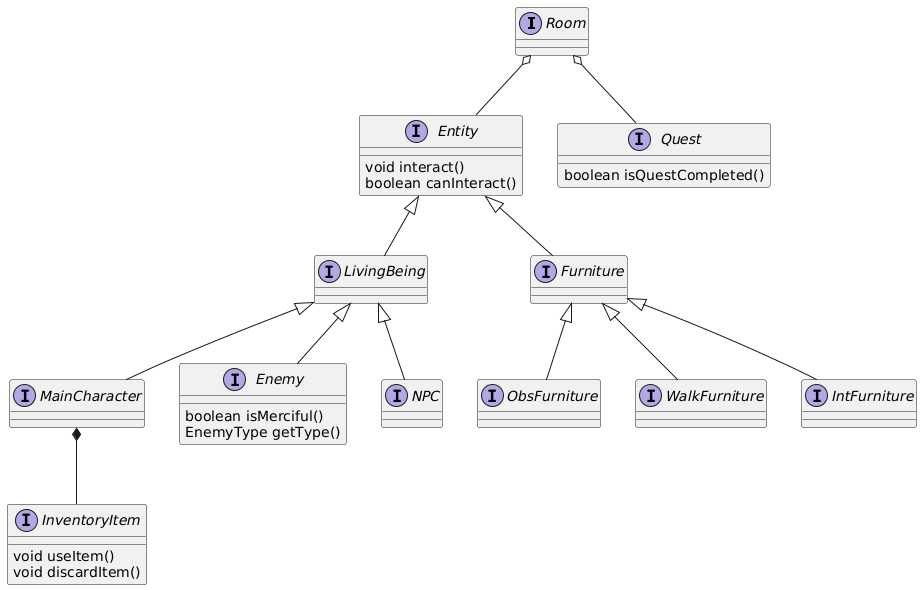
\includegraphics[width=\textwidth]{img/model.png}
	\caption{Schema UML del dominio applicativo}
	\label{img:model}
\end{figure}


\chapter{Design}

\section{Architettura}

Il software si basa sull’architettura MVC nella sua declinazione standard. In particolare, ogni elemento dell’architettura offre un unico entry point verso l’esterno, in modo che gli accessi alle sue funzionalità possano essere uniformi e consistenti, offrendo un ulteriore grado di incapsulamento.
%
\newline Il Model offre come proprio entry point l’interfaccia Room, che fa da scenario base per lo svolgimento della fase di esplorazione del gioco. All’interno della stanza infatti, sono presenti tutte le entità, che vengono modificate ad ogni tick del motore fisico tramite un metodo offerto dalla stessa Room, deputata a controllare anche se le singole entità siano in grado di muoversi al suo interno. 
%
\newline Il Controller, che conserva il riferimento alla stanza in cui attualmente si trova il gioco, gestisce al suo interno le transizioni di stato per le varie fasi del gameplay, interrogando la View per mostrare le interfacce corrette e richiedendo al Model eventuali modifiche. Il Controller è anche responsabile della temporizzazione dell’aggiornamento del motore di gioco, e della traduzione delle entità del Model in elementi rappresentabili correttamente dalla View.
%
\newline La View offre un entry point centrale da cui è possibile richiedere di mostrare le varie interfacce, o l’accesso ai loro riferimenti per chiamare procedure proprie di tali istanze. Nell’architettura realizzata, la View agisce come elemento passivo ricevendo i dati da mostrare dal Controller tramite opportune interrogazioni. La gestione dell’input permette alla View di comunicare particolari eventi al Controller, che li gestirà e ne rifletterà eventualmente gli effetti sul Model.
%
\newline Nella realizzazione dell’architettura MVC, modificare la View non impatta minimamente il Model, dal momento che è solamente il Controller a dialogare con questa componente. Dall’altro lato, il Controller potrebbe essere impattato da una modifica della View radicale (come per esempio trasformare la GUI attiva in un’interfaccia reattiva, oppure la rimozione dei suoni), mentre non sarebbe impattato da modifiche nelle tecniche implementative della GUI - come per esempio una modifica della libreria grafica - a patto che sia in grado di rispettare il contratto stabilito dalle due interfacce (ad esempio accettare gli stessi tipi di chiamate parametrizzate).


\begin{figure}[H]
	\centering{}
	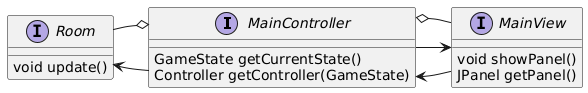
\includegraphics[width=\textwidth]{img/mvc.png}
	\caption{Schema UML degli entry point dei rapporti fra componenti di MVC}
	\label{img:mvc}
\end{figure}

\section{Design dettagliato}

\subsection{Lorenzo Cinelli}
Mi sono occupato della realizzazione del controllo di collisioni e interazioni tra i living being e le altre entità presenti nella stanza, 
dell'interfaccia utente per l'inventario, delle scene di transizione tra le varie fasi di gioco, della visualizzazione di animazioni durante il combattimento
e della gestione dei suoni e canzoni per le varie fasi del gioco.

\textbf{Collisioni e Interazioni}
Il giocatore e gli altri esseri viventi possono muoversi all'interno di una stanza ma non possono coesistere 
contemporaneamente nello stesso punto della stanza insieme ad un altro essere vivente o a una parte di arredamento (non calpestabile).
Il giocatore e gli altri esseri viventi possono interagire con un'entità (che può essere un altro essere vivente o un pezzo di arredamento)
di fronte ad egli. 
Il controllo delle collisioni, che decreta se il movimento del soggetto è consentito oppure no, deve quindi prendere in considerazione
tutti gli esseri viventi presenti in mappa, l'arredamento e la dimensione della stanza e verificare che il soggetto si muoverà in un posto consentito.
Il controllo delle interazioni, che decreta se ci si trova di fronte ad un'entità interattiva, prende in considerazione
tutti gli esseri viventi presenti in mappa e l'arredamento. 
È stata fatta la scelta di evitare di avere interazioni attive da parte delle entità non giocanti (NPC), di conseguenza solo il protagonista interagirà
attivamente con le varie entità, tuttavia con la stessa soluzione sarebbe possibile avere interazioni attive anche da parte degli altri esseri viventi.
IMMAGINE
PATTERN

\textbf{GUI Inventario}
Il giocatore durante il gioco e specialmente durante i combattimenti ha la necessità di interagire con gli oggetti
che ha ottenuto. 
L'inventario è guidato da input da tastiera che vengono gestiti tramite un key listener. Questi vengono passati al
controller dell'inventario che implementa la classe Observer. Il controller si occupa di applicare le modifiche arrivate tramite
l'evento di input all'inventario e riflette queste modifiche nella visualizzazione grafica, aggiornandola coi dati più recenti.
Per facilitare la creazione dell'interfaccia grafica è stata utilizzata una factory per la creazione dei vair componenti
interni della GUI.
IMMAGINE
PATTERN Observer e Factory.

\textbf{Scene di transizione}
Le scene di transizione riguardano l'introduzione, i passaggi da una stanza all'altra e gli scenari riguardanti la fine del gioco.
La scena iniziale ha lo scopo di introdurre il gioco spiegandone l'obiettivo. Gli scenari della fine del gioco possono essere due
differenti in caso di vittoria - dati in base a come la vittoria è stata ottenuta - oppure quello di sconfitta, in caso non si riesca
a vincere la battaglia finale contro il re.
Le scene vengono chiamate in base allo stato del gioco da show() nell'apposito controller. Le scene sono temporizzate, ed al termine
di questo tempo terminano con la chiamata al controller del metodo progress() per passare alla fase di gioco successiva, specificando
a quale fase passare.
IMMAGINE
PATTERN

\textbf{Animazioni di combattimento}
Le animazioni di combattimento vengono mostrate qualora il protagonista o un nemico sferri un attacco. 
IMMAGINE
PATTERN

\textbf{Gestione dei suoni}
La gestione dei suoni passa da un sound locator, che prende le risorse e le trasforma in clip, e poi ogni clip è gestita internamente
alla singola view in cui viene eseguita. 
Inizialmente l'idea era di avere un'unica classe che gestisse interamente i suoni, tuttavia questo portava a dei problemi esponendo
la rappresentazione interna della classe, quindi ho optato per gestire i singoli oggetti all'interno delle rispettive view. 
I suoni sono suddivisi in colonne sonore ed effetti. Le colonne sonore sono differenti per il menu iniziale, per le stanze e per i combattimenti
- con una dedicata al combattimento col boss - mentre gli effetti sono presenti durante l'avanzamento di stanza, durante le animazioni di combattimento
e dirante le scene di fine gioco - separando la vittoria dalla sconfiitta.
IMMAGINE
PATTERN


\chapter{Sviluppo}
\section{Testing automatizzato}

Per quanto riguarda il testing automatizzato, si è sfruttata la libreria JUnit e si sono realizzati test su quasi tutte le classi di Model e Controller. Ciò è stato fatto per garantire il corretto funzionamento dell’applicazione, e per avere la certezza che gli eventuali problemi riscontrati durante il gioco non fossero dovuti a mancanze di logica implementativa, quanto a problematiche di visualizzazione. 
%
\newline La View, invece, è stata testata manualmente in fase di sviluppo, e poi in fase di collaudo del software, perché personalmente non siamo riusciti ad approfondire le dinamiche di testing automatizzato che avrebbero permesso di testare automaticamente anche quella parte del software.
%
\newline In linea generale, gli aspetti su cui il testing si è maggiormente soffermato sono stati i seguenti:

\begin{itemize}
	\item Generazione della mappa, movimento e interazioni al suo interno. Particolarmente, si è verificato che il movimento e le interazioni non generassero comportamenti imprevisti e che si riflettessero correttamente sugli aggiornamenti del Model.
	\item Combattimento. In particolare, il testing si concentra sul mantenimento dell’ordine dei turni per evitare comportamenti imprevisti, e sul corretto inserimento in inventario del bottino dei nemici sconfitti.
	\item Protagonista. In particolare, si è testato il sistema di gestione della vita del protagonista, così come del suo inventario. Nei controlli sull’inventario, si è verificato il corretto utilizzo degli oggetti curativi, così come delle armi e armature, per garantire comportamenti consistenti in fase di combattimento.
	\item Input utente. Si sono testati i Controller che svolgono la funzione di Observer, per garantire la corretta gestione degli input.
	\item Creazione delle istanze. Avendo fatto largo uso del Pattern Factory, si è deciso di testare i metodi di generazione degli oggetti per verificare l’effettiva consistenza delle istanze create e garantire prevedibilità in fase di gioco.
\end{itemize}

\section{Note di sviluppo}

\subsection{Lorenzo Cinelli}

\begin{itemize}
	\item \textbf{Espressioni Lambda:} Utilizzate nella classe \textit{InventoryControllerImpl} nei metodi \textit{notify} e \textit{regress} per gestire rispettivamente
	gli eventi osservati sul key listener ed il cambio di stato del gioco in uscita dall'inventario.
	Permalink: \url{https://github.com/KimboCoffee/OOP23-relario/blob/cb9e0fd37a803cebfb509ff1b08d7df99b5ee8fc/src/main/java/it/unibo/oop/relario/controller/impl/InventoryControllerImpl.java#L57-L77}
	Permalink: \url{https://github.com/KimboCoffee/OOP23-relario/blob/cb9e0fd37a803cebfb509ff1b08d7df99b5ee8fc/src/main/java/it/unibo/oop/relario/controller/impl/InventoryControllerImpl.java#L138-L142}
	\item \textbf{Stream ed espressione Labmda:} Utilizzati nella classe \textit{InventoryControllerImpl} nel metodo \textit{getItemsNames} per restituire una lista di stringhe
	da una lista di oggetti di inventario.
	Permalink: \url{https://github.com/KimboCoffee/OOP23-relario/blob/cb9e0fd37a803cebfb509ff1b08d7df99b5ee8fc/src/main/java/it/unibo/oop/relario/controller/impl/InventoryControllerImpl.java#L83-L86}
	\item \textbf{Optional:} Utilizzati nella classe \textit{InventoryItems} nel metodo \textit{getEquippedItem} per poter passare il campo optional dell'inventario sia per l'armatura
	che per l'arma, i quali possono essere equipaggiati come no.
	Permalink: \url{https://github.com/KimboCoffee/OOP23-relario/blob/cb9e0fd37a803cebfb509ff1b08d7df99b5ee8fc/src/main/java/it/unibo/oop/relario/model/inventory/InventoryItems.java#L33-L34}
	\item \textbf{Reflection:} Utilizzata nella classe \textit{InventoryItems} nel metodo \textit{getDurability} per controllare se l'oggetto di inventario passato sia un oggetto
	equipaggiabile, e di conseguenza se ha una durabilità.
	Permalink: \url{https://github.com/KimboCoffee/OOP23-relario/blob/cb9e0fd37a803cebfb509ff1b08d7df99b5ee8fc/src/main/java/it/unibo/oop/relario/model/inventory/InventoryItems.java#L51}
	\item \textbf{Espressioni Lambda:} Utilizzate nella classe \textit{CutSceneControllerImpl} nei metodi \textit{show}, \textit{progressGame} e \textit{progressView} utilizzate
	rispettivamente per mostrare la scena corretta in base allo stato del gioco, caricare il controller successivo mentre viene mostrata la scena e mostrare la view successiva in
	base allo stato successivo una volta terminata la scena.
	Permalink: \url{https://github.com/KimboCoffee/OOP23-relario/blob/cb9e0fd37a803cebfb509ff1b08d7df99b5ee8fc/src/main/java/it/unibo/oop/relario/controller/impl/CutSceneControllerImpl.java#L27-L56}
	\item \textbf{Espressioni Lambda:} Utilizzate nelle classi \textit{CutSceneViewImpl}, \textit{CombatScene} e \textit{CombatAnimationImpl} per indicare l'azione da far eseguire ai timer una volta scaduti.
	Permalink: \url{https://github.com/KimboCoffee/OOP23-relario/blob/cb9e0fd37a803cebfb509ff1b08d7df99b5ee8fc/src/main/java/it/unibo/oop/relario/view/impl/CutSceneViewImpl.java#L84}
	Permalink: \url{https://github.com/KimboCoffee/OOP23-relario/blob/cb9e0fd37a803cebfb509ff1b08d7df99b5ee8fc/src/main/java/it/unibo/oop/relario/view/impl/CutSceneViewImpl.java#L94-L97}
	Permalink: \url{https://github.com/KimboCoffee/OOP23-relario/blob/cb9e0fd37a803cebfb509ff1b08d7df99b5ee8fc/src/main/java/it/unibo/oop/relario/view/impl/CutSceneViewImpl.java#L114-L117}
	Permalink: \url{https://github.com/KimboCoffee/OOP23-relario/blob/cb9e0fd37a803cebfb509ff1b08d7df99b5ee8fc/src/main/java/it/unibo/oop/relario/view/impl/CutSceneViewImpl.java#L128-L131}
	Permalink: \url{https://github.com/KimboCoffee/OOP23-relario/blob/cb9e0fd37a803cebfb509ff1b08d7df99b5ee8fc/src/main/java/it/unibo/oop/relario/view/impl/CombatScene.java#L117}
	Permalink: \url{https://github.com/KimboCoffee/OOP23-relario/blob/cb9e0fd37a803cebfb509ff1b08d7df99b5ee8fc/src/main/java/it/unibo/oop/relario/view/impl/CombatAnimationImpl.java#L55}
	\item \textbf{Espressione Lambda:} Utilizzata nella classe \textit{CombatAnimationImpl} nel costruttore per gestire la risorsa da utilizzare come animazione.
	Permalink: \url{https://github.com/KimboCoffee/OOP23-relario/blob/cb9e0fd37a803cebfb509ff1b08d7df99b5ee8fc/src/main/java/it/unibo/oop/relario/view/impl/CombatAnimationImpl.java#L46-L50}
\end{itemize}

Le classi \textit{ImageLocators} e \textit{SoundLocators}, per caricare risorse da file, sono state scritte prendendo spunto da Internet.
Permalink: \url{https://github.com/KimboCoffee/OOP23-relario/blob/cb9e0fd37a803cebfb509ff1b08d7df99b5ee8fc/src/main/java/it/unibo/oop/relario/utils/impl/ImageLocators.java#L23-L43}
Permalink: \url{https://github.com/KimboCoffee/OOP23-relario/blob/cb9e0fd37a803cebfb509ff1b08d7df99b5ee8fc/src/main/java/it/unibo/oop/relario/utils/impl/SoundLocators.java#L28-L50}

\chapter{Commenti finali}

In quest'ultimo capitolo si tirano le somme del lavoro svolto e si delineano eventuali sviluppi
futuri.

\textit{Nessuna delle informazioni incluse in questo capitolo verrà utilizzata per formulare la valutazione finale}, a meno che non sia assente o manchino delle sezioni obbligatorie.
%
Al fine di evitare pregiudizi involontari, l'intero capitolo verrà letto dai docenti solo dopo aver formulato la valutazione.

\section{Autovalutazione e lavori futuri}

\subsection{Lorenzo Cinelli}

Sono molto incerto sull'essere soddisfatto o meno di questo progetto, in quanto vedo il mio contributo molto marginale. Ho sempre cercato di dare il massimo sia in fase di analisi,
che di design, progettazione e sviluppo, e sono soddisfatto di ciò che ho fatto, tuttavia ritengo che il carico di lavoro non sia stato minimamente bilanciato, specialmente sulla
suddivisione di Model (che nella pratica non ho avuto). Di fatti appena cominciato a pensare al design della mia parte del progetto mi sono reso conto di avere una parte molto più
ridotta rispetto agli compagni (specialmente nel Model come detto sopra), ma nonostante l'abbia cercato di far notare più volte per provare a suddividere nuovamente e meglio il lavoro
non sono stato preso in considerazione seriamente. 
A causa di questo ritengo anche che questo progetto non mi abbia fatto migliorare quanto mi aspettassi, nonostante comunque abbia imparato molte cose.
Escludendo l'inconveniente della suddivisione del lavoro con gli altri membri del gruppo mi sono trovato molto bene. È stato facile discutere soluzioni implementative e collaborare per
parti comuni.


\section{Difficoltà incontrate e commenti per i docenti}

Permettere la consegna anche durante i periodi di lezione.

\appendix
\chapter{Guida utente}

Capitolo in cui si spiega come utilizzare il software. Nel caso in cui il suo uso sia del tutto
banale, tale capitolo può essere omesso.
%
A tal riguardo, si fa presente agli studenti che i docenti non hanno mai utilizzato il software
prima, per cui aspetti che sembrano del tutto banali a chi ha sviluppato l'applicazione possono non
esserlo per chi la usa per la prima volta.
%
Se, ad esempio, per cominciare una partita con un videogioco è necessario premere la barra
spaziatrice, o il tasto ``P'', è necessario che gli studenti lo segnalino.

\subsection*{Elementi positivi}

\begin{itemize}
 \item Si istruisce in modo semplice l'utente sull'uso dell'applicazione, eventualmente facendo uso di schermate e descrizioni.
\end{itemize}

\subsection*{Elementi negativi}
\begin{itemize}
 \item Si descrivono in modo eccessivamente minuzioso tutte le caratteristiche, anche minori, del software in oggetto.
 \item Manca una descrizione che consenta ad un utente qualunque di utilizzare almeno le funzionalità primarie dell'applicativo.
\end{itemize}

\bibliographystyle{alpha}
\bibliography{13-template}

\end{document}
